% Brechung der Feldlinien an einer dielektrischen Grenzfläche (sigma_f = 0)
% E_t stetig, eps E_n stetig  ->  tan(a1)/tan(a2) = eps1/eps2
% Gemeinsamer Stil für alle Abbildungen (TikZ -> SVG, siehe figures/build.mjs).
%
% Farben sind Platzhalter ("Sentinels"): build.mjs ersetzt sie im SVG durch
% CSS-Variablen, damit die Abbildungen im hellen und dunklen Modus passen.
% Andere Farben (auch schwarz/weiß) bricht der Build mit Fehler ab.
%
%   fg    Linien, Beschriftung          -> --dark
%   mu    Hilfslinien, Achsen, Maße      -> --gray
%   acc   das eine Konzept der Abbildung -> --secondary (Lime/Oliv)
%   blue  zweite Größe, negative Ladung  -> --fig-blue
%   warm  dritte Größe, positive Ladung  -> --fig-warm
%   bg    Seitenhintergrund (Aussparen)  -> --light
%
% Kein \clip verwenden: pdftocairo macht daraus Clip-Gruppen, in denen exakt
% waagerechte/senkrechte Linien verschwinden. Berechnete Kurven schneidet
% gen/*.py selbst am Rahmen ab.
\documentclass[tikz,border=3pt]{standalone}
\usepackage{amsmath,amssymb,bm}
% Text serifenlos wie die Seite, Mathe in Computer Modern wie KaTeX
\renewcommand{\familydefault}{\sfdefault}
\usetikzlibrary{arrows.meta,calc,decorations.markings,patterns,3d,positioning,angles,quotes}

\definecolor{fg}{RGB}{1,2,3}
\definecolor{mu}{RGB}{4,5,6}
\definecolor{acc}{RGB}{7,8,9}
\definecolor{blue}{RGB}{10,11,12}
\definecolor{warm}{RGB}{13,14,15}
\definecolor{bg}{RGB}{16,17,18}

% Vektoren wie auf der Website (KaTeX \mathbf)
\newcommand{\vv}[1]{\mathbf{#1}}

\tikzset{
  every picture/.style={fg, line width=0.8pt, line cap=round, line join=round,
    >={Stealth[length=5.5pt,width=4.4pt]}},
  every node/.style={font=\small},
  % Linientypen
  main/.style={line width=0.9pt},
  thin/.style={line width=0.5pt},
  aux/.style={mu, line width=0.5pt, dash pattern=on 2.5pt off 2pt},
  axis/.style={mu, line width=0.6pt, ->},
  vec/.style={line width=1.1pt, ->},
  field/.style={line width=0.7pt, postaction={decorate},
    decoration={markings, mark=at position #1 with {\arrow{Stealth[length=4.5pt,width=3.6pt]}}}},
  field/.default=0.5,
  % Flächen
  soft/.style={fill=#1, fill opacity=0.14},
  soft/.default=acc,
  % Ladungen
  qpos/.style={circle, fill=warm, inner sep=0pt, minimum size=9pt,
    path picture={\draw[bg, line width=0.9pt] ($(path picture bounding box.center)+(-2pt,0)$) -- +(4pt,0)
      ($(path picture bounding box.center)+(0,-2pt)$) -- +(0,4pt);}},
  qneg/.style={circle, fill=blue, inner sep=0pt, minimum size=9pt,
    path picture={\draw[bg, line width=0.9pt] ($(path picture bounding box.center)+(-2pt,0)$) -- +(4pt,0);}},
  dot/.style={circle, fill=fg, inner sep=0pt, minimum size=3pt},
  % Beschriftung mit Aussparung, damit Linien den Text nicht kreuzen
  lbl/.style={fill=bg, inner sep=1.5pt},
  % Icons: kräftigere Linien, keine Schrift
  icon/.style={line width=1.6pt, >={Stealth[length=6pt,width=5pt]}},
}

\begin{document}
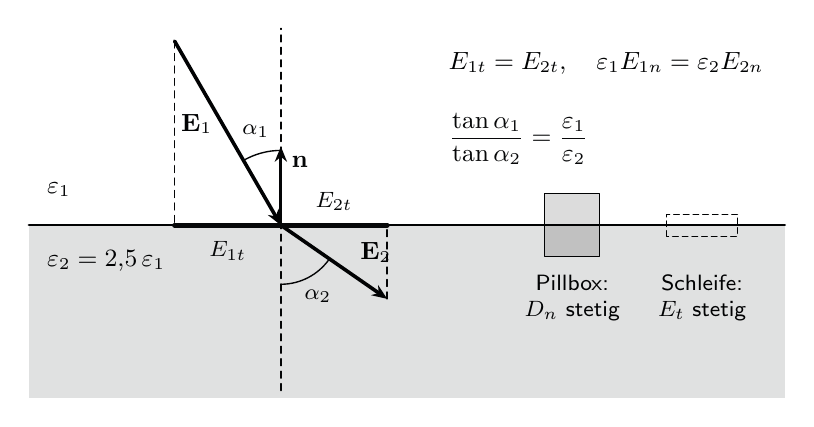
\begin{tikzpicture}
  \def\ea{1} \def\eb{2.5}                 % eps_1, eps_2
  \def\aone{30}                           % Winkel zur Normalen in Medium 1
  \def\Eone{2.7}                          % |E_1| (Zeichenlänge)
  \pgfmathsetmacro{\Et}{\Eone*sin(\aone)}         % tangential, stetig
  \pgfmathsetmacro{\Eonen}{\Eone*cos(\aone)}
  \pgfmathsetmacro{\Etwon}{\Eonen*\ea/\eb}          % eps1 E1n = eps2 E2n
  % Medien
  \fill[mu, fill opacity=0.12] (-3.2,0) rectangle (6.4,-2.2);
  \draw[main] (-3.2,0) -- (6.4,0);
  \node[anchor=west] at (-3.1,0.45) {$\varepsilon_1$};
  \node[anchor=west] at (-3.1,-0.45) {$\varepsilon_2=2{,}5\,\varepsilon_1$};
  \coordinate (O) at (0,0);
  % Normale
  \draw[aux] (0,-2.1) -- (0,2.5);
  \draw[vec, mu] (O) -- (0,1.0) node[anchor=west, text=mu, pos=0.8] {$\vv n$};
  % E_1 kommt von links oben, E_2 läuft nach rechts unten
  \coordinate (A) at ({-\Et},{\Eonen});
  \coordinate (B) at ({\Et},{-\Etwon});
  \draw[vec, line width=1.3pt] (A) -- (O);
  \node[anchor=east] at ($(A)!0.45!(O)$) {$\vv E_1$\ };
  \draw[vec, line width=1.3pt] (O) -- (B);
  \node[anchor=south west] at ($(O)!0.65!(B)$) {$\vv E_2$};
  % Tangentialkomponenten (gleich lang) auf der Grenzfläche
  \draw[aux] (A) -- (-\Et,0);
  \draw[aux] (B) -- (\Et,0);
  \draw[acc, line width=1.8pt] (-\Et,0) -- (0,0);
  \draw[acc, line width=1.8pt] (0,0) -- (\Et,0);
  \node[acc, font=\footnotesize, anchor=north] at ({-\Et/2},-0.08) {$E_{1t}$};
  \node[acc, font=\footnotesize, anchor=south] at ({\Et/2},0.06) {$E_{2t}$};
  % Winkel zur Normalen
  \coordinate (U) at (0,1); \coordinate (D) at (0,-1);
  \pic[draw, mu, thin, angle radius=0.95cm, "$\alpha_1$"{font=\footnotesize, text=mu}, angle eccentricity=1.3] {angle = U--O--A};
  \pic[draw, mu, thin, angle radius=0.75cm, "$\alpha_2$"{font=\footnotesize, text=mu}, angle eccentricity=1.35] {angle = D--O--B};
  % Bedingungen
  \node[anchor=west] at (2.0,2.05) {$E_{1t}=E_{2t},\quad \varepsilon_1E_{1n}=\varepsilon_2E_{2n}$};
  \node[anchor=west, acc] at (2.0,1.1) {$\dfrac{\tan\alpha_1}{\tan\alpha_2}=\dfrac{\varepsilon_1}{\varepsilon_2}$};
  % Pillbox und Schleife
  \begin{scope}[shift={(3.7,0)}]
    \draw[fg, thin, soft=mu] (-0.35,-0.4) rectangle (0.35,0.4);
    \node[font=\footnotesize, align=center, anchor=north] at (0,-0.5) {Pillbox:\\$D_n$ stetig};
    \draw[fg, thin, dash pattern=on 2pt off 1.5pt] (1.2,-0.14) rectangle (2.1,0.14);
    \node[font=\footnotesize, align=center, anchor=north] at (1.65,-0.5) {Schleife:\\$E_t$ stetig};
  \end{scope}
\end{tikzpicture}
\end{document}
